\documentclass[a4paper, 14pt]{extarticle}

% Поля
%----------------------
\usepackage{geometry}
\geometry{a4paper,left=2cm,right=1cm,
    top=2cm,bottom=2cm,bindingoffset=0cm}
%----------------------

% Russian-specific packages
%----------------------
\usepackage[T2A]{fontenc}
\usepackage[utf8]{inputenc}
\usepackage[english, main=russian]{babel}
%----------------------

\usepackage{textcomp}

% Красная строка
%----------------------
\usepackage{indentfirst}
%----------------------

% Graphics
%----------------------
\usepackage{graphicx}
\graphicspath{ {./images} }
\usepackage{wrapfig}
%----------------------

% Import minted
%----------------------
\usepackage{minted}
%----------------------

\linespread{1.3}
\sloppy
\clubpenalty=10000
\widowpenalty=10000



\begin{document}

%--------------------------------------
%			ТИТУЛЬНЫЙ ЛИСТ
%--------------------------------------
\begin{titlepage}
\thispagestyle{empty}
\newpage


%Шапка титульного листа
%--------------------------------------
\vspace*{-60pt}
\hspace{-65pt}
\begin{minipage}{0.3\textwidth}
\hspace*{-20pt}\centering

\includegraphics[width=\textwidth]{emblem}
\end{minipage}
\begin{minipage}{0.67\textwidth}\small \textbf{
\vspace*{-0.7ex}
\hspace*{-6pt}\centerline{Министерство науки и высшего образования Российской Федерации}
\vspace*{-0.7ex}
\centerline{Федеральное государственное бюджетное образовательное учреждение }
\vspace*{-0.7ex}
\centerline{высшего образования}
\vspace*{-0.7ex}
\centerline{<<Московский государственный технический университет}
\vspace*{-0.7ex}
\centerline{имени Н.Э. Баумана}
\vspace*{-0.7ex}
\centerline{(национальный исследовательский университет)>>}
\vspace*{-0.7ex}
\centerline{(МГТУ им. Н.Э. Баумана)}}
\end{minipage}
%--------------------------------------

%Полосы
%--------------------------------------
\vspace{-25pt}
\hspace{-35pt}\rule{\textwidth}{2.3pt}

\vspace*{-20.3pt}
\hspace{-35pt}\rule{\textwidth}{0.4pt}
%--------------------------------------

\vspace{1.5ex}
\hspace{-35pt} \noindent \small ФАКУЛЬТЕТ\hspace{80pt} <<Информатика и системы управления>>

\vspace*{-16pt}
\hspace{47pt}\rule{0.83\textwidth}{0.4pt}

\vspace{0.5ex}
\hspace{-35pt} \noindent \small КАФЕДРА\hspace{50pt} <<Теоретическая информатика и компьютерные технологии>>

\vspace*{-16pt}
\hspace{30pt}\rule{0.866\textwidth}{0.4pt}
  
\vspace{11em}

\begin{center}
\Large {\bf Лабораторная работа № 2} \\ 
\large {\bf по курсу <<Языки и методы программирования>>} \\
\large <<Разработка простейшего класса на языке Java>> \\
\large Вариант 8
\end{center}\normalsize

\vspace{8em}


\begin{flushright}
  {Студент группы ИУ9-22Б Павлов И. П. \hspace*{15pt}\\ 
  \vspace{2ex}
  Преподаватель Посевин Д. П.\hspace*{15pt}}
\end{flushright}

\bigskip

\vfill
 

\begin{center}
\textsl{Москва 2023}
\end{center}
\end{titlepage}
%--------------------------------------
%		КОНЕЦ ТИТУЛЬНОГО ЛИСТА
%--------------------------------------

\newpage
\section{Цель работы}
Целью данной работы является изучение базовых возможностей языка Java. 

\section{Условие}
Каждый публичный класс в языке Java должен размещаться в отдельном файле, базовая
часть имени которого совпадает с именем класса. В данной лабораторной работе потребуется
разработать два класса: основной класс, реализующий функциональность в соответствии с
вариантом задания, и вспомогательный класс, демонстрирующий работоспособность
основного класса. 

\section{Реализация основного класса}
{\small 
\begin{minted}{java}
public class Vector {
    private double x, y, z;

    public double getX() {
        return this.x;
    }

    public double getY() {
        return this.y;
    }

    public double getZ() {
        return this.z;
    }

    public String printVector() {
        return "(" + this.x + ", " + this.y + ", " + this.z + ")";
    }

    public Vector(double x, double y, double z) {
        this.x = x;
        this.y = y;
        this.z = z;
    }

    public double scalarProd(Vector b) {
        return this.x * b.x + this.y * b.y + this.z * b.z;
    }

    public Vector vectorProd(Vector b) {
        double i = this.y * b.z - this.z * b.y;
        double j = this.z * b.x - this.x * b.z;
        double k = this.x * b.y - this.y * b.x;
        return new Vector(i, j, k);
    }

    public boolean isOrthogonal(Vector b) {
        return this.scalarProd(b) == 0;
    }

}
\end{minted}
}

\section{Реализация второстепенного класса}
{\scriptsize
\begin{minted}{java}
public class Main {

    public static void main(String[] args) {
        Vector a = new Vector(2, 3, 5);
        Vector b = new Vector(6, 3, 4);

        double scProd = a.scalarProd(b);
        System.out.println("Скалярное произведение двух векторов: " + scProd + "\n");

        Vector vProd = a.vectorProd(b);
        System.out.println("Координаты вектора, полученного векторным произведением:" + vProd.printVector() + "\n");
        System.out.println("Координата x: " + vProd.getX());
        System.out.println("Координата y: " + vProd.getY());
        System.out.println("Координата z: " + vProd.getZ());

        boolean isOrth = a.isOrthogonal(b);
        if (isOrth) {
            System.out.println("\nВекторы ортогональны.");
        } else {
            System.out.println("\nВекторы не ортогональны.");
        }
    }

}
\end{minted}
}

\begin{figure}[h] 
\center{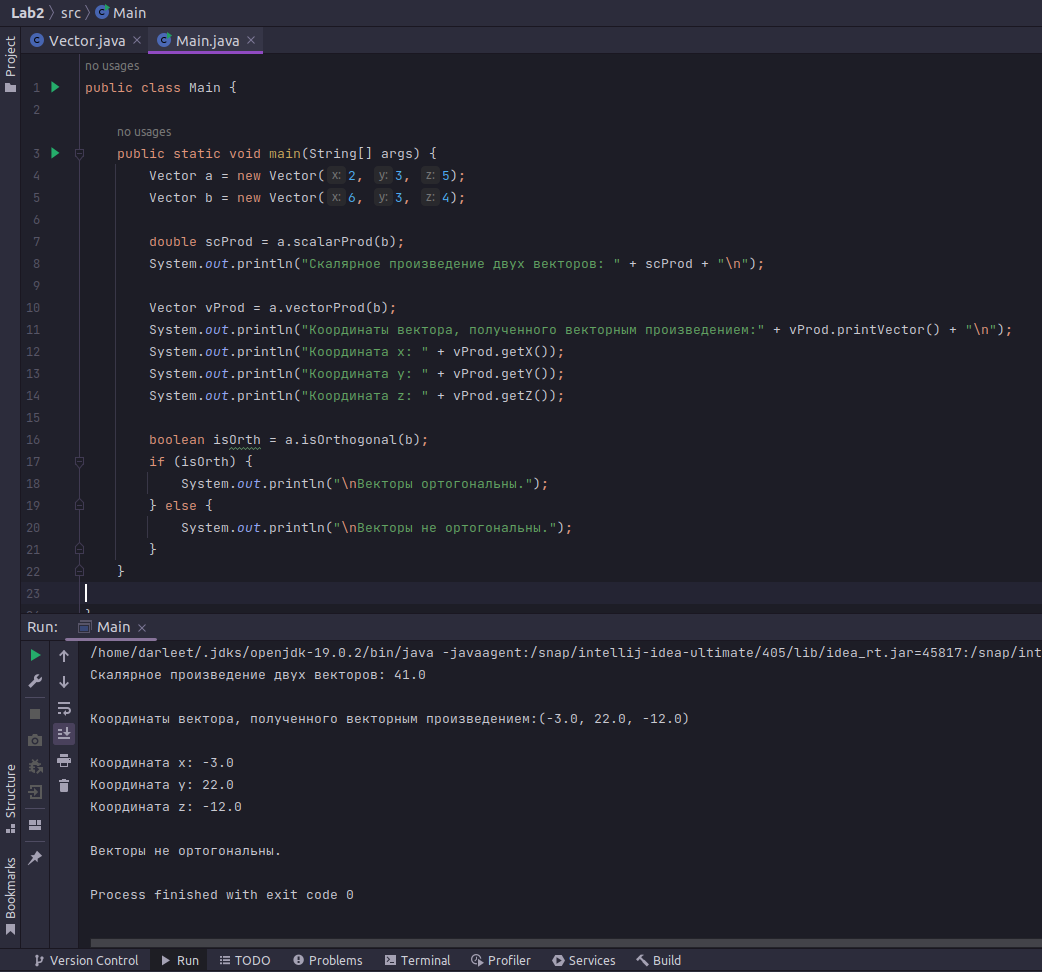
\includegraphics[scale=0.5]{class_main.png}} 
\caption{Вывод программы} 
\label{fig:image} 
\end{figure}

\end{document}
